\documentclass{ieeeaccess}
\usepackage[T1]{fontenc}
\usepackage{cite}
\usepackage{amsmath,amssymb,amsfonts}
\usepackage{amsthm}
\usepackage{algorithm}
\usepackage{algorithmic}
\usepackage{graphicx}
\usepackage{textcomp}
\usepackage{subfigure}
\usepackage{color}
%\usepackage{caption}
\renewcommand{\algorithmicrequire}{\textbf{Input:}}
\renewcommand{\algorithmicensure}{\textbf{Output:}}
\usepackage{bm}
\usepackage{booktabs}
\newcommand{\tabincell}[2]{\begin{tabular}[t]{@{}#1@{}}#2\end{tabular}}
% \newtheorem{definition}{Definition}
\theoremstyle{definition}
\newtheorem{defn}{Definition}

\def\BibTeX{{\rm B\kern-.05em{\sc i\kern-.025em b}\kern-.08em
    T\kern-.1667em\lower.7ex\hbox{E}\kern-.125emX}}

\begin{document}
\history{Date of publication xxxx 00, 0000, date of current version xxxx 00, 0000.}
\doi{10.1109/ACCESS.2017.DOI}

\title{A Hierarchical Feature Selection Method for Network Anomaly Detection}
\author{\uppercase{Jiewen Mao},
\uppercase{Yongquan Hu, Dong Jiang, Tongquan Wei, and Fuke Shen}}
\address{School of Computer Science and Technology, East China Normal University, Shanghai 200062, China}

\markboth
{J. Mao \headeretal: A Hierarchical Feature Selection Method for Network Anomaly Detection}
{J. Mao \headeretal:A Hierarchical Feature Selection Method for Network Anomaly Detection}

\corresp{Corresponding author: Tongquan Wei (e-mail: tqwei@cs.ecnu.edu.cn).}

\begin{abstract}
    Abnormal detection of network traffic is still an important means of preventing network attacks. In the anomaly detection process, researchers need to deal with a large number of features in network traffic. In order to determine whether the network traffic is the most essential feature of the attack, in this paper we propose a hierarchical feature selection method. The method selects the essential features of network traffic through feature clustering method based on correlation coefficient and feature ranking method based on information gain, then it classifies network traffic by decision tree classifier. Experiments show that our method reduces the number of features, and shortens training time comparing with full feature set. By comparison with chi-square feature selection method, our method improves the metrics including accuracy, precision, recall and F1-score.
\end{abstract}

\begin{keywords}
    feature selection, abnormal detection, feature clustering, correlation coefficient, information gain, decistion tree
\end{keywords}

\titlepgskip=-15pt

\maketitle

\section{Introduction}
\label{sec:introduction}
\IEEEPARstart{W}{hile} the Internet of Things, 5G technology, the improvement of network bandwidth and new network security testing tools bring convenience to people, malicious traffic and network attacks are still serious threats to Internet users and servers. 
On March 2015, GitHub faced a massive DDoS attack. The attack lasted for one week and caused significant damages\cite{github-2015}. On October 2016, Dyn's DNS servers was attacked for two hours, during that time, internet users directed to Dyn servers were unable to reach some of the marquee brands of the internet\cite{dyn-2016}. On May 2017, the WannaCry ransomware attack bursted and over 200,000 compromised computers across 150 countries were influenced by this virus and economic losses from the cyber attack could reach up to 4 billion dollars\cite{wannacry-2017}.

Traditional anomaly detection methods often only use the header information of the network packets. Wang et.al. \cite{Wang2020CS} proposed a dynamic MLP-based attack detection method. The feature selection process of this paper uses backward selection filter method. It deletes the features which make the accuracy of MLP decreasing more than threshold and the remainings are the selected features. However the method in \cite{Wang2020CS} only uses the header information including source IP, TCP flag, source port, destination port, etc.. Urmila et al.\cite{Urmila2017} a Distributed collaboration detection scheme that combines the advantages of Anomaly and Signature based method by capturing the packet header in real time. AL-Hawawreh\cite{MunaSulieman2017} discussed the SYN flood attack in virtual cloud and detects it based on new features that extracted from TCP/IP header. Alsharafi et al.\cite{Alsharafi2020} investigates a Normal Profile Updating Method (NPUM) for enhancing the PHAD based IDS model, which updates normal profile of anomaly IDS using further processing of both the normal and abnormal data identified by anomaly detector.
However, diverse types of network anomalies cannot be distinguish effectively only by packet header information. Even in some types of attacks the malicious users may construct and send the packets elaborately to escape the detection from intrusion detection systems(IDS). Once these packets pass the prevension and propagate in the network, the target computer or network device will be compromised.
To solve this problem, this paper takes the statistical information extracted by aggregated flows besides the header information. Different types of anomalies have different statistical patterns. For example, (D)DoS attacks may have larger counts of packets but stable flow duration, while in brute-force attack the packet counts will be smaller but the curve of flow duration fluctuates drasticly. 

Another problem of statistical detection methods are dimensional explosion. A flow may have more than 30 features in the header alone. Considering the statistical characteristics of all packets in flows, number of features in a network data set will grow rapidly. There may be linear relationships or other associations between these features. If we take all features into consideration, on one hand the efficient of learning and modeling algorithms will decrease, on the other hand it is hard to find the intrinsic cause that can determine whether a flow is an attack.

This paper proposes a hierarchical feature selection method, including three steps of data preprocessing, feature clustering and feature ranking. First, we preprocess the network traffic data. This procedure includes removing features that are clearly not available for statistical analysis, filling or dropping missing data, and encoding labels to numerical values. Second, we propose a feature clustering algorithm based on Pearson correlation coefficient to cluster the features with strong correlation and then select the cluster center. The third step will continue the second step, a feature rank algorithm based on information gain and information gain ratio is used to further filter the features. Finally, we use the decision tree (DT) as a classifier and conduct experiments among our proposed method, the features selected by chi-square testing algorithm and the full feature set. We compare them by the training time and training metrics including accuracy, precision, recall and F1-score. 

The contributions of our paper can be summarized as follow:

\begin{enumerate}
    \item This paper proposes a feature clustering method based on Pearson correlation coefficient, which uses correlation coefficients to define distances and aggregates the features with similar distances, and finds the cluster center as the representative feature of the cluster.
    \item This paper proposes a feature ranking algorithm based on information gain, which sorts the features selected before and choose top $k$ features as the final result of selector.
    \item This paper then analyzes the selected feature subset and explains why they can determine whether a flow is normal or attack.
    \item This paper uses decision tree as classifier to compare selected feature subset using proposed method, chi-square selection method, and the complete feature set on the aspect of training time, accuracy, precision, recall and F1-score.
\end{enumerate}

The remaining part of the paper is organized as follows: Section \ref{sec:related} describes related works. Section \ref{sec:problem} describe the formalization of feature selection problem. Section \ref{sec:methods} introduces our hierarchical feature selection method. Section \ref{sec:evaluation} shows the experiment results and the discussion about the results. Finally Section \ref{sec:conclusion} concludes this paper and indicates future works.

\section{Related Works}
\label{sec:related}

Different approaches have been proposed to apply to feature selection to improve the performance of feature selection. H. C. Law et al. propose an expectation-maximization (EM) algorithm to estimate the importance of different features and the best number of components for Gaussian-mixture clustering\cite{Law2004}. EM can avoid running EM many times with different numbers of components and different feature subsets, and can achieve better performance than using all the available features for clustering. Yang et al.\cite{Yang2018} present a modified Network Maximal Correlation (NMC) model as a measure to capture correlation relationships between a characteristic variable and a label variable. The results show the method can obtain an optimal subset of features with faster speed, maximum correlation and minimal redundancy through numerical simulation.

In addition, various of new feature selection approaches have been presented in the past years. Wu et al. \cite{Wu2017}propose a new feature selection algorithm based on features unit (FU), which uses entropy of information to obtain features units and sort them to selected the appropriate one. The results in the UCI datasets show that the FU performs better than MIFS-U and mRMR on the whole. Yassine et al.\cite{Yassine2017} propose a new hybrid filter-wrapper algorithm of feature selection based on pairwise feature selection, which benefits from the speed up and the ease of use of filters and the good performance of wrappers. The results indicate that the selected subset of features by the proposed approach has a good classification performance. Yang et al. \cite{Yang2018a} propose a novel unsupervised feature selection method where constructing similarity matrix and performing feature selection are together incorporated into a coherent model. The results show the proposed approach has better performance to solve the objective function and extensive experiments on face images and benchmark datasets. Ke et al. \cite{Ke2018} propose a redundant window-based optimal feature subset discover algorithm for feature selection, which use the growth algorithm to discover the relevant features and use the shrink algorithm to eliminate the redundant ones. The results show that the method has a good performance in terms of accuracy and scalability, and improves the execution efficiency of feature selection and traffic classification.

Liu et al. \cite{Liu2018} propose a differentially private ensemble feature selection algorithm based on output perturbation. The results also demonstrate the high performance under certain privacy preservation degree of the method. Ferriyan et al. \cite{Ferriyan2017} propose a new feature selections using Genetic Algorithm to find the optimal features from NSL-KDD Cup 99 dataset, which use one-point crossover for the Genetic Algorithm parameters instead of two-point crossover. The results show the proposed approach performs better in classification rate and the training time compared to several other classifiers. Han et al. \cite{Han2020} propose a novel unsupervised feature selection method via the graph matrix learning and the low-dimensional space learning to obtain their individually optimized result. The results on real datasets verified that the method achieved the best classification performance compared to the state-of-the-art feature selection methods.

Feature selection also have been broadly used in processing traffic data. Shi et al. \cite{Shi2017} propose a novel feature extraction and selection approach to provide the optimal and robust features for traffic classification, which based on multifractal features, the observation of the multifractal features and the analysis of PCABFS. The results show the approach achieves better classification performance, lower runtime performance and more effective for real-time traffic classification compared to the TLS features. Moreover, the authors then propose a new feature optimization approach based on deep learning and Feature Selection (FS) techniques\cite{Shi2018} to provide the optimal and robust features for traffic data sets. The results show the approach achieves the best classification performance and relatively higher runtime performance compared with the approaches used in the previous work.

Moreover, there are different feature selection methods aim to process different kinds of data. Dong et al.\cite{Dong2017} propose a fine grained classification scheme which based on a hierarchical kNN classifier for network video traffic. The results show that the proposed method outperforms existing methods applying commonly used flow statistical features. Taskin et al. \cite{Taskin2017} presented a novel feature-selection method based on High Dimensional Model Representation (HDMR) to analyze and test in classification of hyperspectral images. The results show that the proposed approach can be used as a fast and efficient feature-selection method yielding very competitive results compared to the state-of-art feature-selection methods. Valadi et al.\cite{Valadi2019} propose a new modification of attribute selection with multiple label which can be advantageously used for handling high dimensional multi-level datasets. The results show the proposed approach reduces complexity and computational run time.

% \begin{figure*}[!htbp]
%     \centering
%     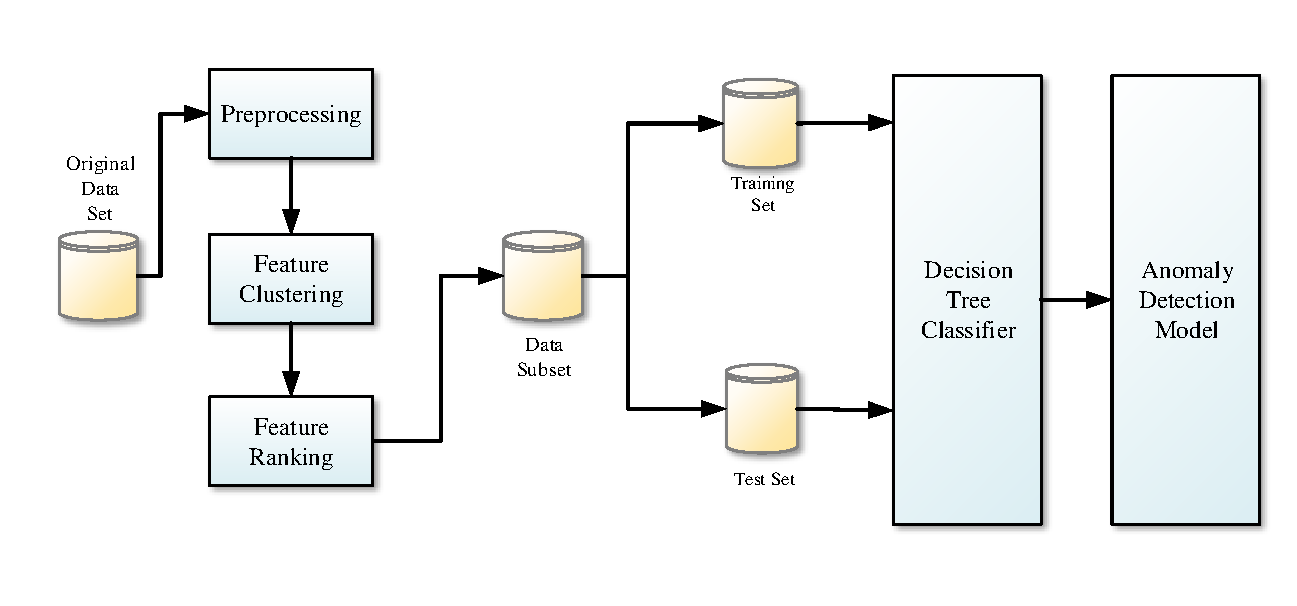
\includegraphics[scale=0.8]{fig/Framework.pdf}
%     \caption{Detection Framework}
%     \label{fig:framework}
% \end{figure*}
\Figure[t!](topskip=0pt, botskip=0pt, midskip=0pt)[scale=0.8]{fig/Framework.pdf}{Detection Framework\label{fig:framework}}

\section{Problem Definition and Solution}
\label{sec:problem}
We denote 
$$D=\left(\begin{array}{llll}
    \bm{x}_1 & \bm{x}_2 & \ldots & \bm{x}_m
\end{array}\right)^T$$
as the data set with $m$ instances, where 
$$\bm{x}_i = \left(\begin{array}{lllll}
    f_{1i} & f_{2i} & \ldots & f_{ni} & c_i
\end{array}\right)$$
where $f_{ji}$ is the value of $j$th feautre of vector $\bm{x_i}$, and $f_j \in F = \{f_1, f_2, \ldots, f_n\}$ is the feature set. $c_i$ is the class label of $\bm{x}_i$ and $c_i \in C = \{c_1, c_2, \ldots, c_k\}$, where $C$ is the set of class labels.

The feature selection problem\cite{Maza2018} can be described as a 6-tuple $FS=\langle D, F, C, S, fs, E \rangle$, where $D, F, C$ are data set, feature set and class label set respectively. $S=\{s_1, s_2, \ldots, s_l\}, \ l=2^n-1$ is the search space, which contains all subsets can be constructed from $F$ with $s_i=\{f_j, f_k, \ldots, f_l\}, \ (1 \leqslant j \neq k \neq l \leqslant n)$. $E$ is the evaluation measure and $fs$ represents the function of process of feature selection: $fs: F \rightarrow S$.

The target of the function $fs$, which is the proposed algorithm, is to find the best feature subset $\hat{F} \subset F$. The feature subset should satisfy following conditions:
\begin{itemize}
    \item Every feature $f \in \hat{F}$ is independent with others. It means that every $f$ should not be calculated from other features.
    \item The feature subset $\hat{F}$ is the least set of $s_l$ with given count of features $l$. This feature subset should has enough information to determine whether a flow is an attack or not. If the feature set add or remove any other features, the result of detection will deteriorate.
\end{itemize}

To find such feature subset, we propose our hierarchical feature selection algorithm, which is presented in next Section.

\section{Hierarchical Feature Selection Method}
\label{sec:methods}

In this section, we explain our design of proposed hierarchical feature selection method in turn. First of all is the overview and structure of our method. Then the source of data set and preprocessing procedure are introduced. Next we explain our feature clustering algorithm and feature ranking algorithm respectively. After that we simply introduce decision tree classifier, which is used as our model-building tools. Finally, we compare the difference of the theory of our method and dimensionality reduction algorithms like PCA.

\subsection{Overview}

The system framework of this paper is shown as Fig. \ref{fig:framework}. 
The proposed method is the first block in the figure, and it contains three steps or layers: The first step is preprocessing, which cleans data set and makes it to a better form to be processed in next two steps. The second step is feature clustering, which puts all features with potential linear correlation into the same cluster, then all cluster centers are chosen as the representative of every clusters. The third step is feature ranking, which further rank all features selected in step 2 and choose the top $k$ features as the final feature set. 

After the three-steps processing, the refined data subset is divided into training set and test set, then they are trained and tested via decision tree classifier and our detection model is generated.

In following subsections the details and algorithms of proposed methods are described.

\subsection{Data Set and Preprocessing}

The data set being studied is CIC-IDS-2018\cite{cic2018}. 
It is generated on a simulated network topology on the AWS computing platform. The network topology is shown as Figure \ref{fig:topology}. It has 5 subnet and 1 attacker network.  
The data set consists of seven different attack scenarios: Brute-force, Heartbleed, Botnet, DoS, DDoS, Web attacks, and infiltration of the network from inside. It includes the captured network traffic and system logs of each machine, along with 76 features extracted from the captured traffic using CICFlowMeter-V3\cite{cicflowmeter}. These 76 features are shown in Table \ref{tab:features}.

% \begin{figure}[!htbp]
%     \centering
%     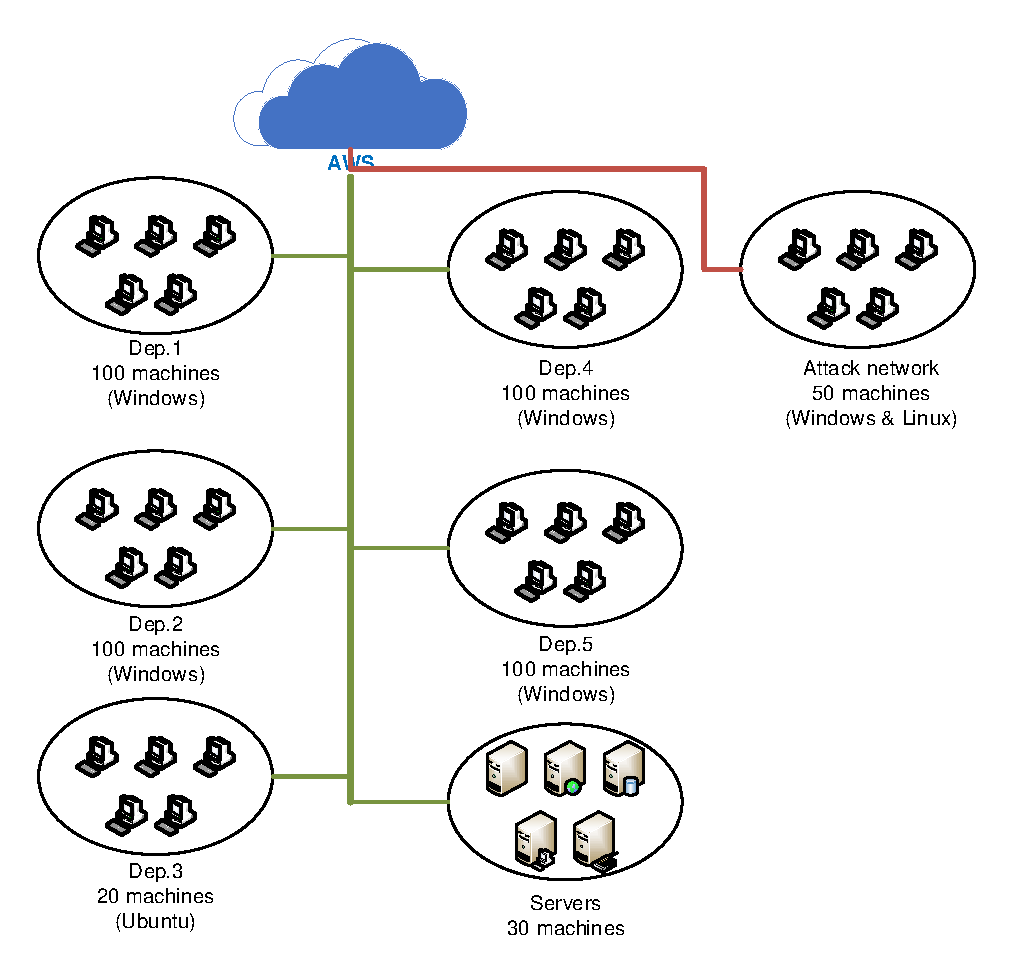
\includegraphics[scale=0.5]{fig/Topology.pdf}
%     \caption{Simulated network topology on AWS computing platform}
%     \label{fig:topology}
% \end{figure}
\Figure(topskip=0pt, botskip=0pt, midskip=0pt)[scale=0.45]{fig/Topology.pdf}{Simulated network topology on AWS computing platform\label{fig:topology}}

\begin{table*}[!htpb]
    \caption{76 Features of CIC-IDS-2018 data set}
    \label{tab:features}
    \centering
    \begin{tabular}{llll}
    \toprule
    \multicolumn{4}{c}{Features} \\
    \midrule
    Flow Duration & Total Forward Packets & Total Backward Packets & Total Length Forward Packets \\
    Total Length Backward Packets & Forward Packet Length Max & Forward Packet Length Min & Forward Packet Length Mean \\
    Forward Packet Length Std & Backward Packet Length Max & Backward Packet Length Min & Backward Packet Length Mean \\
    Backward Packet Length Std & Flow Bytes/s & Flow Packets/s & Flow IAT Mean \\
    Flow IAT Std & Flow IAT Max & Flow IAT Min & Forward IAT Total \\
    Forward IAT Mean & Forward IAT Std & Forward IAT Max & Forward IAT Min \\
    Backward IAT Total & Backward IAT Mean & Backward IAT Std & Backward IAT Max \\
    Backward IAT Min & Forward PSH Flags & Backward PSH Flags & Forward URG Flags \\
    Backward URG Flags & Forward Header Length & Backward Header Length & Forward Packets/s \\
    Backward Packets/s & Packet Length Min & Packet Length Max & Packet Length Mean \\
    Packet Length Std &  Packet Length Var & FIN Flag Count & SYN Flag Count \\
    RST Flag Count & PSH Flag Count & ACK Flag Count & URG Flag Count \\
    CWE Flag Count & ECE Flag Count & Down/Up Ratio & Packet Size Avg \\
    Forward Seg Size Avg & Backward Seg Size Avg & Forward Byts/b Avg & Forward Packets/b Avg \\
    Forward Blk Rate Avg & Backward Byts/b Avg & Backward Packets/b Avg & Backward Blk Rate Avg \\
    Subflow Forward Packets & Subflow Forward Byts & Subflow Backward Packets & Subflow Backward Byts \\
    Init Forward Win Byts &  Init Backward Win Byts &   Forward Act Data Packets & Forward Seg Size Min \\
    Active Mean & Active Std & Active Max & Active Min \\
    Idle Mean & Idle Std & Idle Max & Idle Min \\
    \bottomrule
    \end{tabular}

\end{table*}

In order to detect all types of attacks as much as possible, we integrated the network traffic data that was originally scattered in each day, and extracted 20\% of the data as our main data set while maintaining the label ratio. At the same time, in order to ensure the generalization ability of the model, we randomly select and generate data sets as many times as possible. Finally we get 10 stratified-sampled data set files. 

At this moment, the data set is still unavailable because there are some useless nominal features which are not suitable for statistical analyzing, and there may be missing values in the data set. We must remove these features to prevent them interfering proposed algorithms.

Our preprocessing strategy is described as follows:

\subsubsection{Data cleaning}
The target of this paper is to find the decisive statistical features which can determine whether a network flow is an attack. 
So the traditional 5-tuple, i.e. source IP address, source port, destination IP address, destination port and protocol cannot be used to our algorithm. 
These nominal features will be removed to focus on other statistical features. 
We also remove timestamp feature because our algorithm focuses on the type of attacks rather than the time characteristics.

Many missing values also exist in the data set. There are many reasons for missing values. Some flows cannot be calculated in certain features. For example, if the duration time of a flow is too small even equals 0, the values of two features named ``Flow Bytes/s'' and ``Flow Packets/s'' can be NaN or infinity. It is a difficult work to examine every missing value, and they cannot be filled using interpolation because the data set is composed randomly. In this situation, we remove these rows containing missing values to ensure our algorithm running normally.

Note that the removed features are only in the context of this paper. These features may be useful in other detection methods.

\subsubsection{Remove all zero-variance features}

Variance is a physical quantity used to describe the degree of discreteness of a variable. In a data set, if the variance of a feature is zero, it means that this feature has only one value. Thus this feature cannot import any new information to help training the model. We remove these features to refine the data set.

\subsubsection{Encode labels}

Most anomaly detection models perform as classifiers which predict output labels by calculating the probabilities of every label in the label set. The models use input data to train a function. Both input data and output data are often numeric. However in our data set, the labels are text which cannot be processed by detection model. Thus we encoder the labels and map them to numeric values.

\subsection{Layer 1: Feature Clustering Algorithm based on Pearson Correlation Coefficient}

% Many features of the original data set are derived from others. According to our observation, there are linear correlations between many features. The most important step of our method is to merge these linear related features via clustering method. First the concept of correlation coefficient is reviewed.

According to our observation, many features are potentially linear related. For example, in Figure \ref{fig:correlated-variables}, we pick up two pairs of features to show their potential linear correlation. The left part shows that features ``Flow IAT Mean'' and ``Forward IAT Mean'' may have positive correlation. In fact the interval time of a whole flow consists of the forward flow. In the right part, we can see that the feature ``Backward Segment Size Average'' is almost equals to ``Backward Packet Length Mean''. We can treat them as the same feature. 

The redundancy of features is produced by the featrue extraction tool. If we use the whole data set to train our model, the redundant features on one hand may increase the computation and spend more time, on the other hand these redundant features cannot import any new informations into our model. So it is necessary to merge these redundant features. In this paper, we use clustering method to reach this target. 

First the concept of correlation coefficient is reviewed.

\begin{figure}
    \centering
    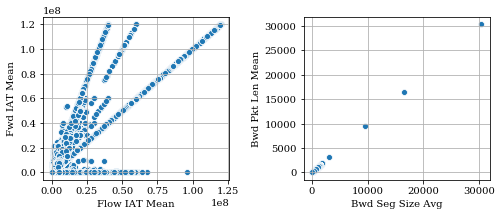
\includegraphics[scale=0.5]{fig/scatter-correlated-variables.png}
    \caption{Two examples of correlated variables. The feature ``Flow IAT Mean'' and ``Forward IAT Mean'', ``Backward Segment Size Average'' and ``Backward Packet Length Mean'' are potentially related. }
    \label{fig:correlated-variables}
\end{figure}

\begin{defn}[Correlation Coefficient]
    If the variances $\sigma^2_X$ and $\sigma_Y^2$ of two random variables $X$ and $Y$ exists and they satisfy that $\sigma^2_X > 0$ and $\sigma^2_Y > 0$, the correlation coefficient of $X$ and $Y$ can be denoted as
\begin{equation}
    \text{Corr}(X, Y) = \frac{\text{Cov}(X, Y)}{\sigma_X \sigma_Y}
\end{equation}
where $\text{Cov}(X, Y)$ is the covariation of $X$ and $Y$. And
$$\text{Corr}(X, Y) \begin{cases}
    > 0, & X \text{ and } Y \text{ are positive correlated.}\\
    = 0, & X \text{ and } Y \text{ are not linear correlated.} \\
    < 0, & X \text{ and } Y \text{ are negative correlated.}
\end{cases}$$
\end{defn}

Then we use the correlation coefficient to define the distance of any two features.

\begin{defn}[The distance of two features]
\label{def:distance}
The distance of two features $f_i$ and $f_j$ is the reciprocal of the absolute value of correlation coefficient of them, that is
\begin{equation}
    \label{eq:distance}
    d(f_i, f_j) = \frac{1}{|\text{Corr}(f_i, f_j)|}
\end{equation}
\end{defn}

According to Equation \ref{eq:distance}, if two features have potential linear correlation, the distance between them is small. On the contrary, if the distance between two features are large, these two features are independent relatively. Here we consider both positive correlation and negative correlation are the same, so we use absolute value of the correlation coefficient. However, the more indepent two features are, the less absolute correlation coefficient of them is. This is the exact opposite of our general definition of distance. Hence we use reciprocal to solve this problem.

The clustering algorithm is described as Algorithm \ref{alg:clustering} and Algorithm \ref{alg:compare-and-join}. We calculate the distance between every feature and others. If the distance is less than a threshold $\delta$, the feature is treated as linear related with the other and they belong to the same cluster. Otherwise, the feature will be put in a new cluster. The procedure ``compare\_and\_join'' at the 4th line of Algorithm \ref{alg:clustering} is complicated, so we list it as Algorithm \ref{alg:compare-and-join}.

\begin{algorithm}
\caption{Feature clustering}
\label{alg:clustering}
\begin{algorithmic}[1]
\REQUIRE ~~\\
    Data set $D=(\bm{x}_1,\bm{x}_2,\ldots,\bm{x}_M)^\text{T}$, \\
    feature set $F=(f_1,f_2,\ldots,f_N)$, \\
    distance threshold $\delta$.
\ENSURE ~~\\
    Cluster set $C=\{c_1,c_2,\ldots,c_K\}$
\STATE $C \gets \emptyset$
\FOR{$i=1,2,\ldots,n$}
    \IF{$\nexists c \in C\ \text{s.t.} f_i \in c$}
        \STATE cluster $c_{join} \gets \text{compare\_and\_join}(D, f_i, C, \delta)$
        \IF{$\exists c_{join}$ which $f_i$ can join}
            \STATE $c_{join}\text{.add}(f_i)$
        \ELSE
            \STATE Create a new cluster $c'$
            \STATE $c'\text{.add}(f_i)$
            \STATE $C\text{.add}(c')$
        \ENDIF
    \ENDIF
\ENDFOR
\RETURN $C$
\end{algorithmic}
\end{algorithm}

\begin{algorithm}
\caption{Compare new feature to all features of all existing cluster}
\label{alg:compare-and-join}
\begin{algorithmic}[1]
\REQUIRE ~~\\
    Data set $D=(\bm{x}_1,\bm{x}_2,\ldots,\bm{x}_M)^\text{T}$, \\
    feature $f_i$, \\
    distance threshold $\delta$,
    currently existing clusters $C=\{c_1, c_2, \ldots, c_K\}$
\ENSURE ~~\\
    A integer $c_{join}$ which indicate the cluster which $f_i$ can join in.  
\STATE A vector including all maximum values of all existing cluster $\bm{d}_{\max}(C) \gets \emptyset$
\FOR{$k=1,2,\ldots,K$}
    \STATE Distance vector for cluster $c_k$, i.e.$\bm{d}(c_k) \gets \emptyset$
    \FOR{$j=1,2,\ldots, \text{sizeof}(c_k)$}
        \STATE $d=\text{Corr}(D^{(f_i)}, D^{(f_j)})|$
        \STATE $\bm{d}(c_k)\text{.add}(d)$
    \ENDFOR
    \STATE $\bm{d}_{\max}(C)\text{.add}(\max{\bm{d}(c_k)})$
\ENDFOR
\STATE Maximum distance in cluster $c_k$ denoted as $d_{\max}=\max{\bm{d}_{\max}(C)}$
\IF{$d_{\max} > \delta$}
    \STATE $c_{join}=\arg\max_c{\bm{d}_{\max}(C)}$
    \RETURN $c_{join}$
\ELSE
    \RETURN NULL
\ENDIF
\end{algorithmic}
\end{algorithm}

Note that in Algorithm \ref{alg:compare-and-join}. We directly use the absolute correlation coefficient instead of complying with the definition of Equation \ref{eq:distance}. This is done because we can limit the range of $\delta$ to $[0,1]$.

After the clusters are generated, next step is to find the center of these clusters. This procedure is listed as Algorithm \ref{alg:find-cluster-center}. We calculate the average distance of every feature between others in each cluster, then we pick the feature with minimum average distance with other features as the center of this cluster. If a cluster only have two features, the algorithm will select the first feature in the cluster as the center of it.

\begin{algorithm}
\caption{Find the cluster center}
\label{alg:find-cluster-center}
\begin{algorithmic}[1]
\REQUIRE ~~\\
    Data set $D=(\bm{x}_1,\bm{x}_2,\ldots,\bm{x}_M)^\text{T}$, \\
    clusters $C=\{c_1, c_2, \ldots, c_K\}$ calculated in Algorithm \ref{alg:clustering}
\ENSURE ~~\\
    A feature list $F'=\{f'_1, f'_2, \ldots, f'_K\}$ whose features are the center of every cluster. 
\STATE Feature list $f'=\emptyset$
\FOR{$i=1,2,\ldots, K$}
    \IF{sizeof($c_i$) = 1}
        \STATE $F'$.add($f \in c_i$)
    \ELSIF{sizeof($c_i$) = 2}
            \STATE select a feature randomly
            \STATE $F'$.add($f \in c_i$)
    \ELSE
        \FOR{each $f \in c_i$}
            \STATE $\bar{d_f}=1/(|c_i|-1)\sum d_{f, f'}$
        \ENDFOR
        \STATE $f_c=\arg\min_f d_c$
        \STATE $F'$.add($f_c$)
    \ENDIF
\ENDFOR
\RETURN $F'$
\end{algorithmic}
\end{algorithm}

\subsection{Layer 2: Feature Ranking Algorithm based on Information Gain}

After the procedure of Layer 1, we generate a group of features which are pairwise independent. In order to further refine the feature space of our data, we choose those have better classification ability. The measure of feature classification ability is the information gain. 

We select the top $k$ best feature using information gain and information gain ratio simultaneously. The related definitions are listed as follows:

\begin{defn}[Entropy of data set]
    Entropy\cite{Shannon1948} is the measure of uncertainty of a random variable. In the context of our paper, the entropy of data set is defined as the entropy of labels. If the probability of label $L$ picking value $l_i$ equals to $P(L=l_i)=p_i$, the entropy of data set is denoted as 
\begin{equation}
    H(D) = -\sum_{i=0}^N p_i \log_2 p_i
\end{equation}
Specially, if $p_i=0$ then we define $0\log0 = 0$. 
\end{defn}

\begin{defn}[Conditional entropy of data set with given feature]
The conditional entropy $H(D|f)$ is the uncertainty of data set $D$ under the condition of known feature $f$, which is denoted as 
\begin{align}
     H(D|f)= & \notag \\
    & -\sum_{j} p(f=f_j) \times \notag \\
    & \sum_{i} p(L=l_i|f=f_j) \log_2 p(L=l_i|f=f_j)   
\end{align}
where $p(f=f_j)$ is the probability when feature $f$ takes $f_j$, $p(L=l_i | f=f_j)$ is the conditional probability when label $L$ takes $l_i$ under the condition of $f=f_j$.
\end{defn}

The information gain indicates the degree to which the uncertainty of the information of the category Y is reduced by the information of the feature X.

\begin{defn}[Information gain]
    The information gain from feature $f$ to data set $D$ is defined as the difference between the entropy $H(D)$ of the set $D$ and the conditional entropy $H(D|F)$ of $D$ for a given feature $f$, i.e.
\begin{equation}
    IG(D, f) = H(D) - H(D|f)
\end{equation}
\end{defn}

Obviously, for data set $D$ the information gain is determined by its features. Different features have different information gain. If a feature has greater information gain, it has stronger ability to classify the data.

\begin{defn}[Information gain ratio]
The problem of using information gain is that it tend to choose the feature which has larger value range. In order to eliminate this effect, the information gain ratio is introduced. It is defined as the information gain divided by entropy of the feature. 
\begin{equation}
    IGR(D, f) = \frac{IG(D, f)}{H(f)}
\end{equation}
\end{defn}

\begin{algorithm}
    \caption{Feature ranking}
    \label{alg:feature-ranking}
    \begin{algorithmic}[1]
    \REQUIRE ~~\\
        Data set $D'$ with clustered features calculated in Algorithm \ref{alg:clustering} and \ref{alg:find-cluster-center}
    \ENSURE ~~\\
        A feature list $F''=\{f''_1, f''_2, \ldots, f''_k\}$ whose features are top $k$ after ranked. 
    \STATE Calculate the entropy $H(D')$ by its labels.
    \FOR{$i=1,2,\ldots, K$}
        \STATE Calculate the conditional entropy $H(D'|f_i)$.
        \STATE Calculate the information gain $$IG_{f_i} = H(D') - H(D'|f_i)$$
        \STATE Calculate the information gain ratio 
        $$IGR_{f_i} = IG_{f_i}/H(f_i)$$
    \ENDFOR
    \STATE Calculate the average information gain $\bar{IG}=(\sum IG) / K$
    \STATE Choose the features $F_{IG}=\{f|IG_{f} > \bar{IG}\}$
    \STATE Sort the features according to $IGR$
    \RETURN $F''$
    \end{algorithmic}
    \end{algorithm}

Now our feature ranking algorithm is introduced in Algorithm \ref{alg:feature-ranking}. We consider the information gain and information gain ratio simultaneously. First we calculate the information gain of all features which has been clustered by Algorithm \ref{alg:clustering} and \ref{alg:find-cluster-center}. Then we calculate the average information gain and sort them by their information gain ratio. Finally we select top $K$ features to compose new feature set. Here we set $K=10$. In different anomaly detection scenarios, the value of $K$ should be chosen on demand.



\subsection{Decision Tree Classifier}

Since we have selected all features we need to determine whether a flow is an attack. Furthermore we want to detect detailed attack types. We choose C4.5 decision tree\cite{quinlan2014c4} as our classification algorithm. C4.5 decision tree uses information gain ratio to classify data instances. The implementation of decision tree algorithms is beyond the scope of this article. However, our method in fact previously complete the feature selection process of decision tree, so the tree classifier can use our result and speed the training process.

\subsection{Compare to Dimensionality Reduction Algorithms}

Our method is one kind of feature selection algorithm. It is different from dimensionality reduction algorithms like PCA\cite{PCA1987}. PCA transforms the original data into a set of linearly independent representations of each dimension by linear transformation to extract the main linear components of the data, while feature selection methods do not transform the data. It just chooses the key features which can provide the most information about the data. The data transformed by PCA will lose their explanation of real meaning, while feature selection algorithms can keep the real meaning of every reserved features. 

Meanwhile, our proposed method includes some characteristics of PCA. First, we calculate the covariance and correlation coefficient of all feature vectors, which is also used in calculation of PCA. Second, the features selected by our method are orthogonal and PCA do the same thing. Last but not least, every component generated by PCA have maximum variance, and our method contains the similar step. But in our method, the features with small variance are filtered.

\section{Experiment results}
\label{sec:evaluation}

In this section, the experiments and evaluation results are shown. First we describe the experiment setup. Then we list selected feature by our algorithm and explain why these feature are selected. Next, since the distance threshold $\delta$ is a changeable parameter, we describe how the numbers of clusters are impacted by different distance threshold. Further, we compare the training time and classification metrics including accuracy, precision, recall and F1-score between our method and the full original data set, as well as our method and Select K Best method based on chi-square function respectively. Finally we illustrate and explain the confusion matrix of our prediction results.

\subsection{Experiment Setup}

All experiments are running on a quad-core Intel PC with 2.90GHz CPU and 16 GB of memory. Our algorithms are implemented in Python 3.7 and the chi-square method is implemented in a Python library scikit-learn\cite{sklearn}.

\subsection{Selected Feature subset}

Table \ref{tab:selected-features} shows the features selected by our method and their descriptions. Notice that although we set $K=10$ for our feature ranking algorithm, the selected features are not same in all split data set. Because randomicity exists when we build the split data subset. Here we use the union of all selected feature subsets. From Table \ref{tab:selected-features} we make the following observations:

\begin{itemize}
	\item The sizes of packets are important. In the top 10 important features, there are 4 features about packet sizes. Considering the MTU of an IP network, a flow shouldn’t contain too large packets. If the flow meter observes a flow contain large packets, the probability that this stream is an attack stream will be high. 
    \item Another type of important features is the count of packets. In benign flows, the number of packets often small because current network services intend to use short connection to complete the interaction with each other, in order to not occupy the bandwidth resources of the network. However, the attackers intend to send large amounts of packets to exhaust the connection resources and prevent connection from normal users. 
    \item Time-related features are also important. As we mentioned before, benign services intend to use short connection, while attackers may use long connection. A typical attack is to control the interval of any two flows which is a little shorter than the TCP waiting time. It prevents the TCP connection closing and finally exhaust the connection resources. In practise, time-related features should be considered with the count of packets together.
\end{itemize} 

\begin{table}[!htpb]
    \caption{Selected Features and Their Description}
    \label{tab:selected-features}
    \centering
    \begin{tabular}{ll}
    \toprule
        Feature Name    & Description \\
    \midrule
    Backward Packets/s          & \tabincell{l}{Number of backward packets per  \\ second} \\
    Forward Segment Size Min    & \tabincell{l}{Minimum segment size observed in \\ the forward direction} \\
    Init Forward Win Byts   & \tabincell{l}{Number of bytes sent in initial  \\ window in the forward direction} \\
    Flow Packets/s         & \tabincell{l}{flow packets rate that is number of \\ packets transferred per second} \\
    ACK Flag Count        & Number of packets with ACK \\
    Flow IAT Mean       & Average time between two flows \\ 
    Backward IAT Max         & \tabincell{l}{Maximum time between two packets \\ sent in the backward direction} \\
    Idle Mean           & \tabincell{l}{Mean time a flow was idle before \\ becoming active}\\
    Forward Packet Length Min     & \tabincell{l}{Minimum size of packet in forward \\ direction} \\
    Flow Duration       & Flow duration \\
    Backward Packet Length Mean    & \tabincell{l}{Mean size of packet in backward \\ direction} \\
    Packet Length Min         & Minimum length of a flow \\
    Forward Packets/s          & \tabincell{l}{Number of forward packets per  \\ second} \\
    Forward IAT Total         & \tabincell{l}{Totalal time between two packets sent \\ in the forward direction} \\
    \bottomrule
    \end{tabular}
\end{table}

\subsection{Investigate the effect of the distance threshold on the cluster numbers}

In our algorithm, an important parameter is the distance threshold $\delta$. It takes effects on the number of clusters generated in Algorithm \ref{alg:clustering}. Figure \ref{fig:different-threshold} shows the result of number of generated clusters from 10 split data set files under different threshold $\delta$. We set $\delta$ from 0.7 to 0.95 with interval 0.05 between any two values. The average number of clusters are listed in Table \ref{tab:mean-cluster-number}. Here a trade-off exists about the number of clusters and the number of features in every cluster. If $\delta$ is set too small, the number of clusters will be small too, however many features with weak correlation will be merged in the same cluster and it will finally impact subsequent feature ranking and decision tree learning procedures. Meanwhile, a larger $\delta$ will produce too many clusters which contains only one feature, because the condition is too stricted to merge features. In our practice, setting $\delta$ between 0.8 and 0.9 is a better choicce.

\begin{figure}
    \centering
    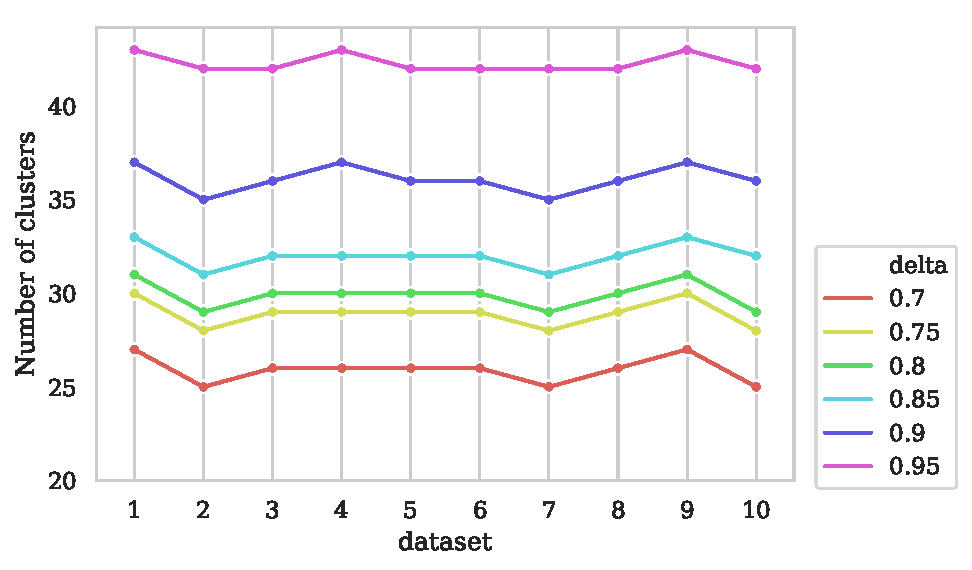
\includegraphics[scale=0.5]{fig/Cluster-Number-in-diff-delta.pdf}
    \caption{Number of clusters in 10 split data set under the effect of different distance threshould $\delta$. }
    \label{fig:different-threshold}
\end{figure}

\begin{table}
    \caption{Average number of clusters under different distance threshold}
    \label{tab:mean-cluster-number}
    \centering
    \begin{tabular}{r|rrrrrr}
        \toprule
        $\delta$ & 0.7 & 0.75 & 0.8 & 0.85 & 0.9 & 0.95 \\
        \midrule
        $\bar{N}$ & 26 & 29 & 30 & 32 & 36 & 42 \\
        \bottomrule
    \end{tabular}
\end{table}

\subsection{Compare with training time and metrics on full original data set}

In this subsection we compare the training time of decision tree classifier and the metrics of classification effects between our method under different distance threshold $\delta$ and the full original data set.

\subsubsection{Training Time}

The training time in our method is the sum of running time of all algorithms mentioned before. The training time under different distance threshold $\delta$ is shown in Figure \ref{fig:training-time-with-full} and Table \ref{tab:training-time-all}. 
When we use the full original data set to train a decision tree classifier and then prune the tree to 10 decision nodes too, the training time is near 300 seconds averagely. Using our method, the training time decreases near 100 seconds averagely.  
Meanwhile this figure shows that the average training time increases slowly with $\delta$ increasing.

\begin{table}[!htbp]
    \centering
    \caption{Training Time comparing to full data set and chi-square method}
    \label{tab:training-time-all}
    \begin{tabular}{lr}
        \toprule
        dataset & Training Time(s) \\
        \midrule
        $\delta=0.7$ & 264.70 \\
        $\delta=0.75$ & 266.21 \\
        $\delta=0.8$ & 265.12 \\
        $\delta=0.85$ &  267.21 \\
        $\delta=0.9$ &   269.39 \\
        $\delta=0.95$ & 269.89 \\
        Full data set & 308.14 \\
        Select K Best ($\chi^2$) & 103.36 \\
        \bottomrule
    \end{tabular}
\end{table}


\begin{figure}[!htpb]
    \centering
    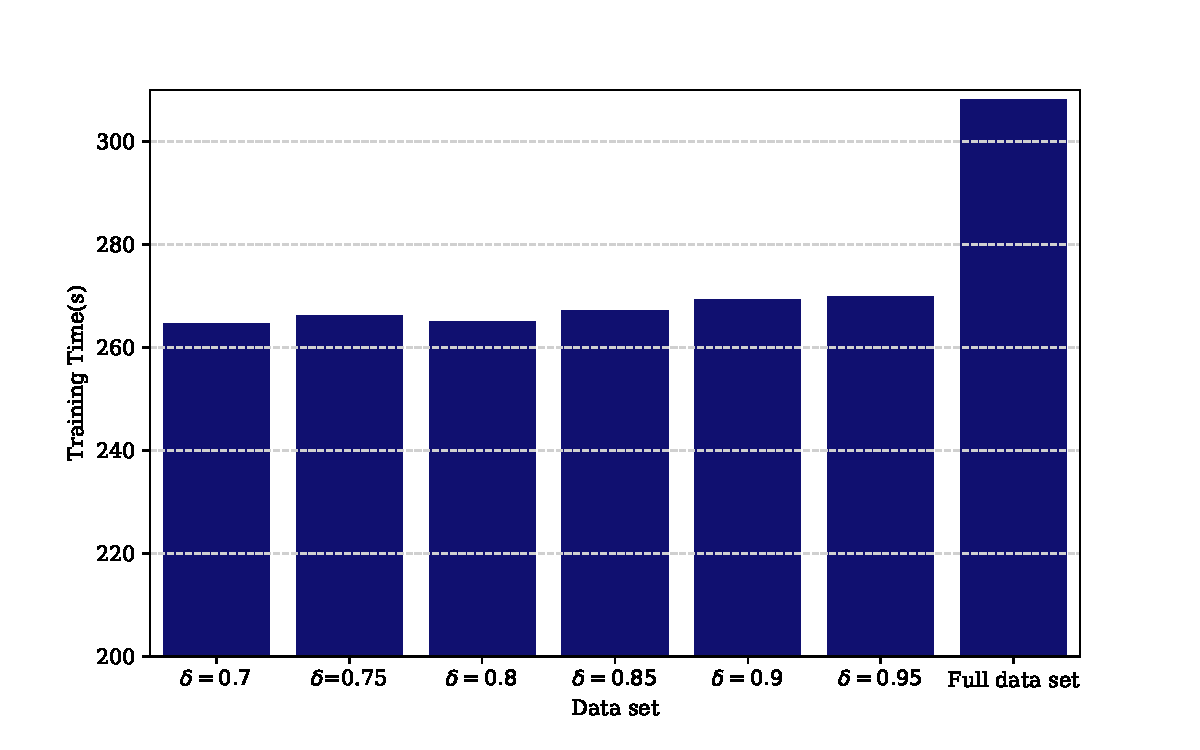
\includegraphics[scale=0.45]{fig/training-time-all.pdf}
    \caption{Training Time comparison with full original data set}
    \label{fig:training-time-with-full}
\end{figure}

\subsubsection{Metrics}

The metrics of model include accuracy, precision, recall and f1-score. Related definitions are listed below:

\begin{defn}[Accuracy]
    In classification problems, we denote $TP$ as true positve prediction, $FP$ as false positive prediction, $TN$ as true negative prediction and $FN$ as false negative prediction.

    The accuracy is defined as the ratio of $TP+TN$ in all test instances, which is
    \begin{equation}
        \text{Acc}=\frac{TP+TN}{TP+TN+FP+FN}
    \end{equation}
    which means the all true instances classified in all test instances.
\end{defn}

\begin{defn}[Precision]
    The precision is defined as the ratio of $TP$ in all positive instances classified by the model, which is
    \begin{equation}
        \text{Pre} = \frac{TP}{TP+FP}
    \end{equation}
    which means the all true positive instances classified in all positve instances.
\end{defn}

\begin{defn}[Recall]
    The recall is defined as the ratio of $TP$ in all real positive instances, which is
    \begin{equation}
        \text{Rec} = \frac{TP}{TP+FN}
    \end{equation}
\end{defn}

\begin{defn}[F1-score]
    The F1-score is defined as the harmonic average of precision and recall.
    \begin{equation}
        F_1 = \frac{2}{\frac{1}{\text{Pre}} + \frac{1}{\text{Rec}}}
    \end{equation}
    which is a trade-off between the precision and recall.
\end{defn}

These four metrics of our methods under different $\delta$ is shown in Figure , along with the metrics of the model trained on full original data set. The result is shown in Figure \ref{fig:metrics-full} and Table \ref{tab:metric-full}. The average accuracy of our method is 97.94\%, which is a little higher than the accuracy on full data set. The average precision, recall and F1-score are 79.46\%, 80.73\% and 79.33\% respectively. They are all higher than the results on full data set. 

The result proved that the feature selected by our method can help improving performance of decision tree classifier comparing with using tree classifier directly on the full original data set.

\begin{table*}
    \centering
    \caption{The metrics of different $\delta$ and full data set.}
    \label{tab:metric-full}
    \begin{tabular}{lrrrr}
        \toprule
        dataset & Accuracy(\%) & F1-Score(\%) & Precision(\%) & Recall(\%) \\
        \midrule
            $\delta=0.7$ &  97.9604 & 79.0699 & 80.1735 & 79.0867 \\
            $\delta=0.75$ &	97.9297 & 80.2657 & 81.9095 & 79.6229 \\
            $\delta=0.8$ &	97.9104 & 80.2791 & 81.1272 & 80.3653 \\
            $\delta=0.85$ &	97.9558 & 79.3655 & 80.7983 & 79.0457 \\
            $\delta=0.9$ &  97.9557 & 78.9994 & 80.3196 & 78.6552 \\
            $\delta=0.95$ &	97.9489 & 78.8134 & 79.9506 & 79.2532 \\
            Full data set &	97.1315 & 78.0325 & 80.2580 & 77.3223 \\
            Select K Best($\chi^2$) & 94.2846 & 72.1371 & 68.7105 & 69.1960 \\
        \bottomrule
    \end{tabular}
\end{table*}

\begin{figure}[!htpb]
    \centering
    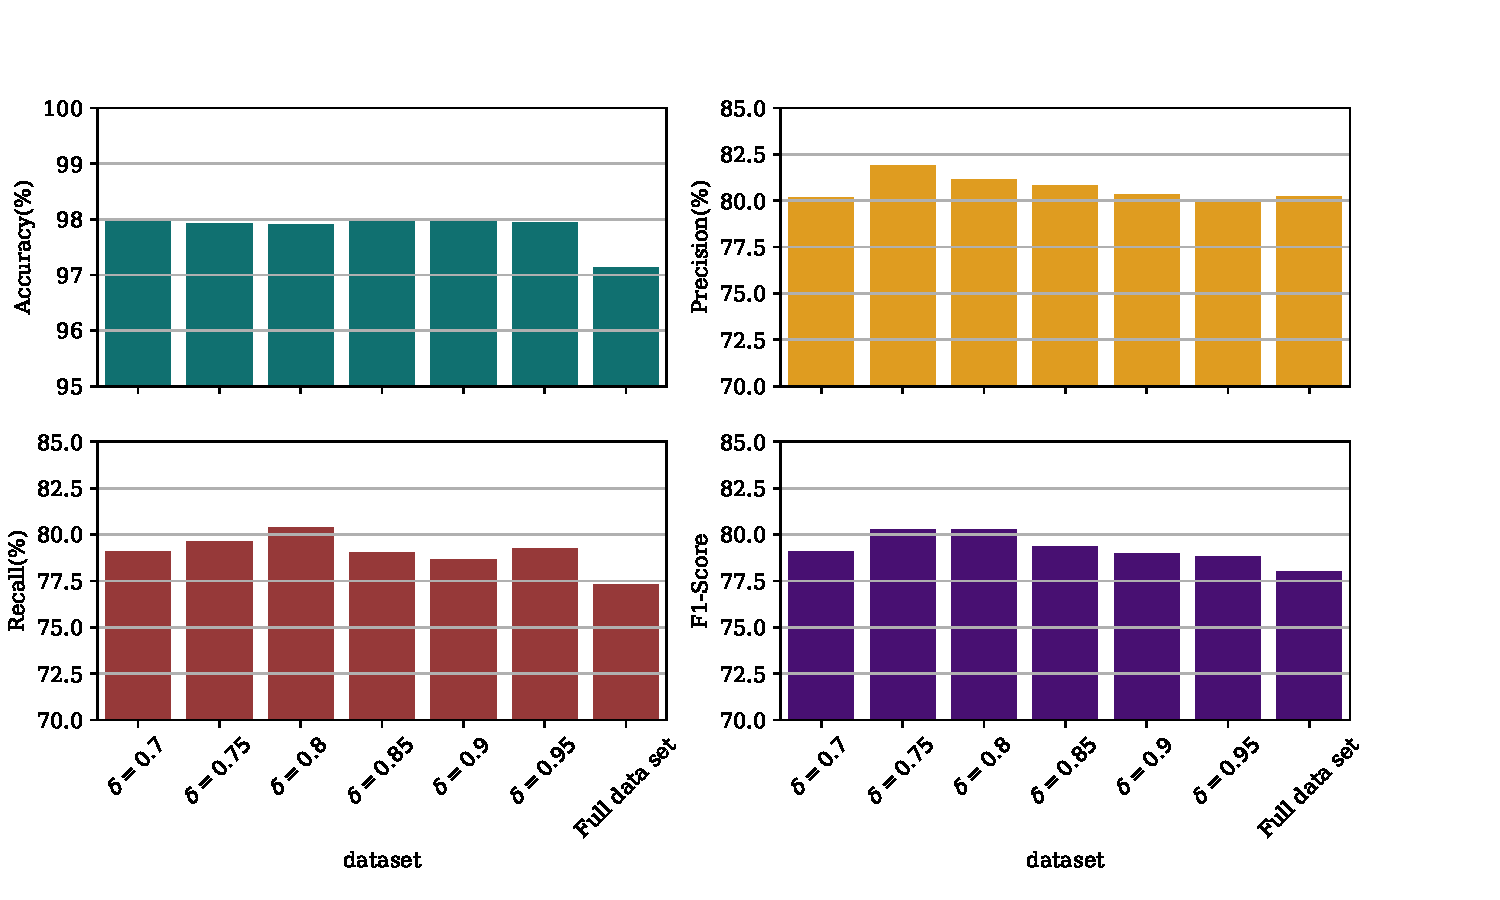
\includegraphics[scale=0.35]{fig/metrics-full.pdf}
    \caption{The metrics including accuracy, precision, recall and F1-score of the data subset with different $\delta$ and the full data set.}
    \label{fig:metrics-full}
\end{figure}

\subsection{Compare with training time and metrics on chi-square-based Select K Best algorithm}

\subsubsection{Training Time}

In this experiment, we compare the training time and metrics of our method and Select-K-Best method using Chi-square funtion in the same size of feature set, in other words the number of features are both set to 10 in these two methods.

The training time comparison is shown in Figure \ref{fig:training-time-with-chi2} and also listed in Table \ref{tab:training-time-all}. We can see our average training time is longer than the chi-square method performs. The chi-square method selects $n$ features with the highest values for the test chi-squared statistic from input data $X$. However, it only considers whether every single feature is correlated with the class label instead of considering the correlation between these features, which makes the training time lower than our methods. 
As a result, the selected feature subset may contain features with inner relationship, which may bring the redundant information in the model. While our method can effectively eliminate the redundant information. 

\begin{figure}[!htpb]
    \centering
    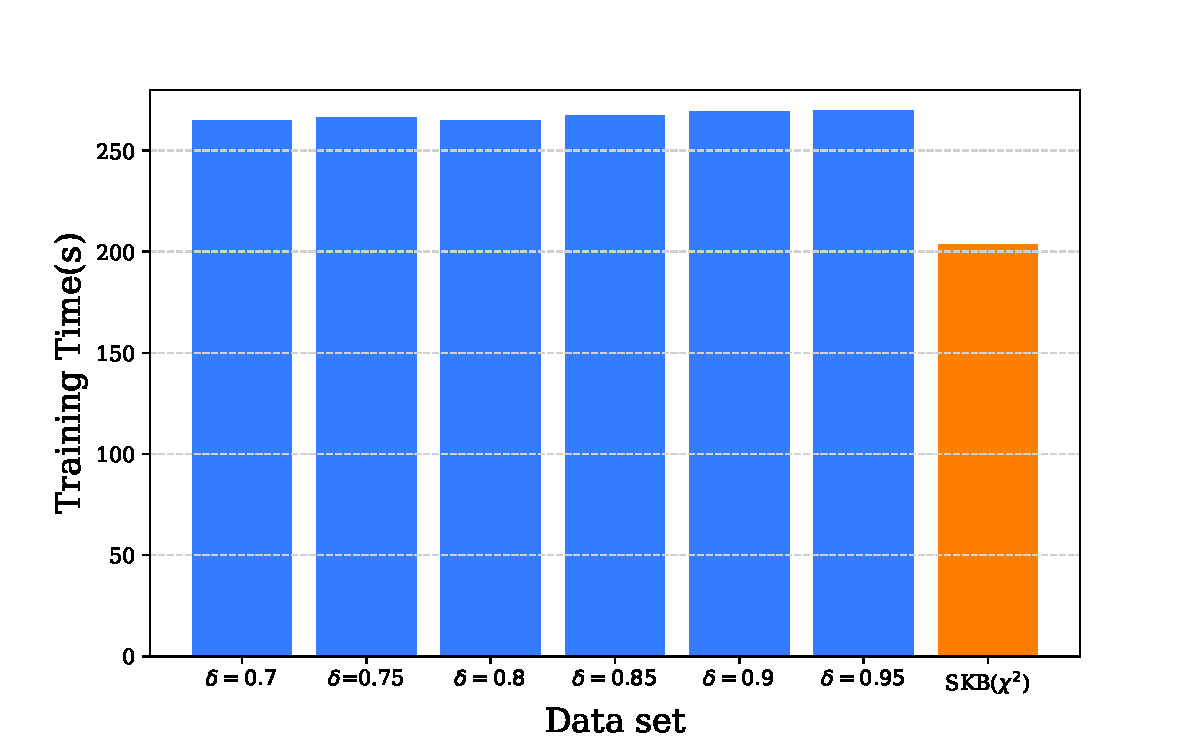
\includegraphics[scale=0.45]{fig/training-time-chi2.pdf}
    \caption{Training Time comparison with full original data set.}
    \label{fig:training-time-with-chi2}
\end{figure}

\subsubsection{Metrics}

The classification metrics comparison is shown in Figure\ref{fig:metrics-chi2} and Table \ref{tab:metric-full}. The figure shows that the metrics of our method are all better than the chi-square funtion. Although the training time is longer, an advantage of our method is that it consider more correlations between any two features comparing with only considering the relationship between any single feature and the class label. Therefore, the experimental results show that our method can better determine the statistical law of traffic when a network attack occurs.

\begin{figure}[!htpb]
    \centering
    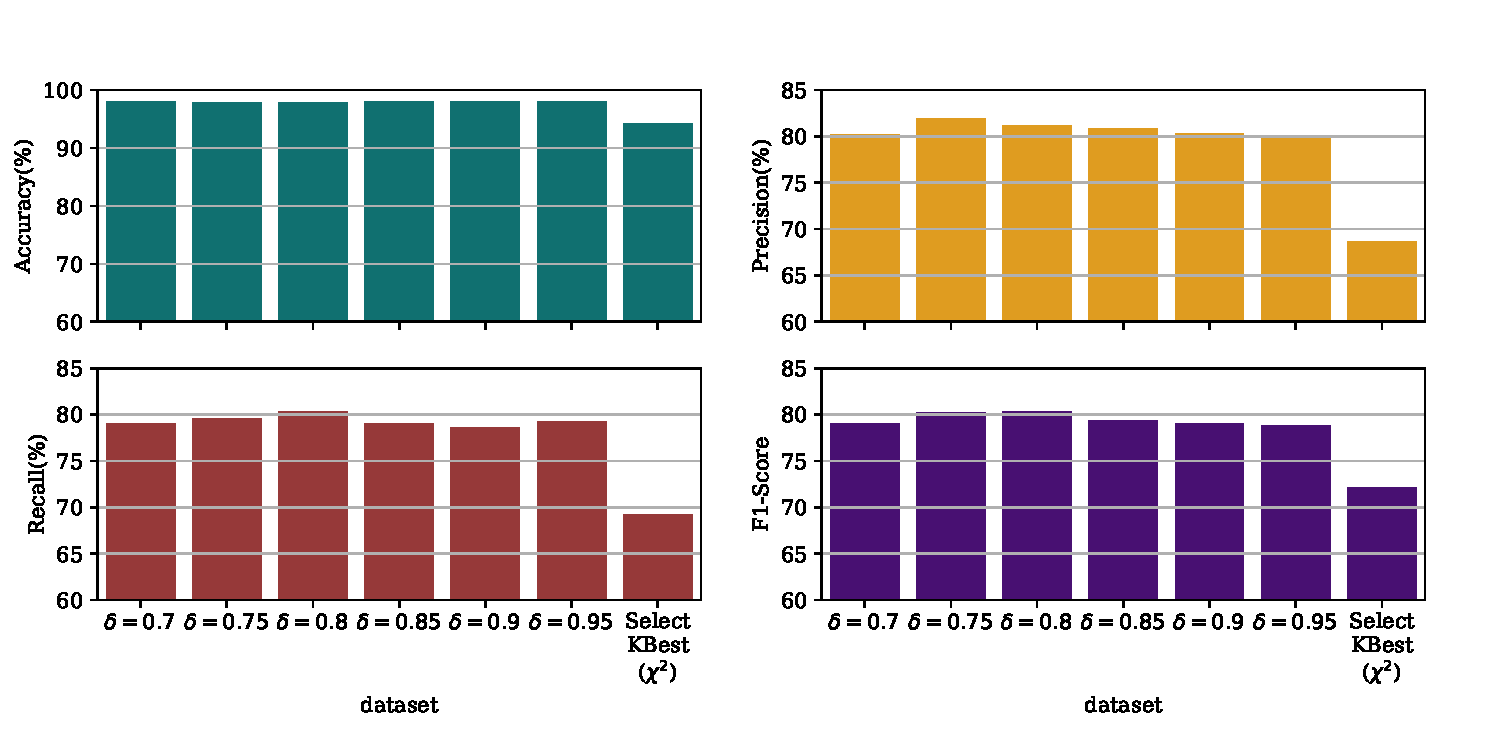
\includegraphics[scale=0.35]{fig/metrics-chi2.pdf}
    \caption{The metrics of the data subset with different $\delta$ and the SelectKBest method based on $\chi^2$ funtion.}
    \label{fig:metrics-chi2}
\end{figure}

\subsection{Confusion Matrix}

Finally we analyze the confusion matrix of our method. The confusion matrix is shown in Figure \ref{fig:confusion-matrix}. We add the confusion matirx of all split data set. The matrix shows that our method can mainly classify the data into correct class label. However, there are still many false positive and false negative instances. The most severe miss happens on the label ``DOS attacks-GoldenEye'' and ``Infilteration''. The flow patterns of these two situation performs similar with benign flow pattern so that our method could not discriminate them properly. The flow patterns of these two situation should be further study and new method should be proposed to detect them.  

\begin{figure*}
    \centering
    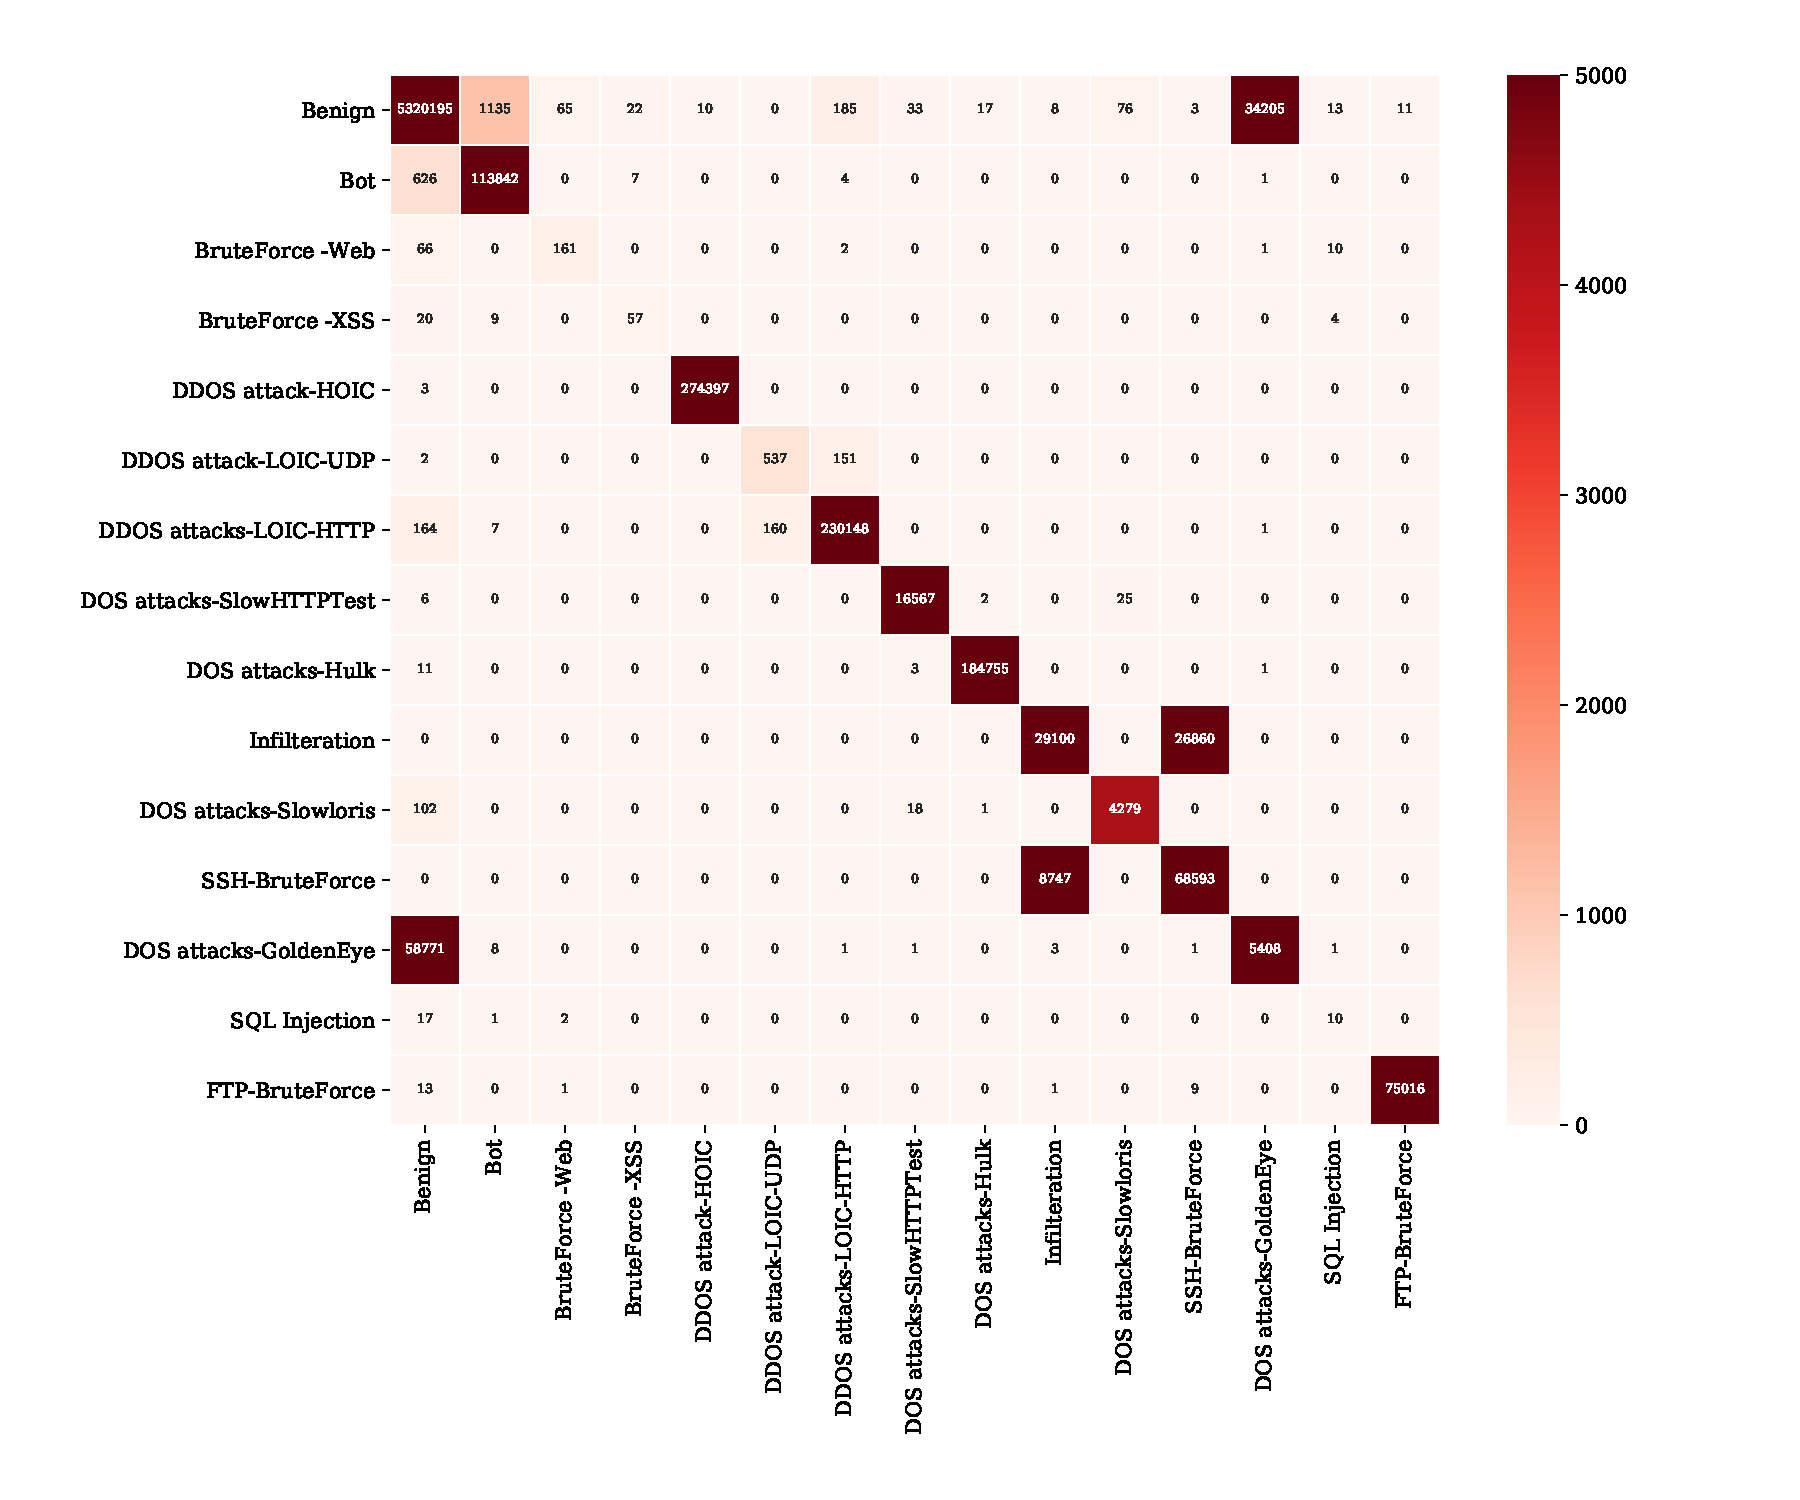
\includegraphics[scale=0.5]{fig/confusion-matrix.pdf}
    \caption{Heatmap of confusion matrix}
    \label{fig:confusion-matrix}
\end{figure*}

\section{Conclusion}
\label{sec:conclusion}

This paper proposed a novel hierarchical feature selection method for network anomaly detection. We applied feature clustering algorithm using correlation-coefficient-based distance between features on network flow traffic data set, then ranked these feature cluster centers using information gain and information gain ratio simultaneously. After that we chose decision tree as our training algorithm to train the model based on the selected feature set. The experiment results shows our method can select more critical features which can determine whether a network flow is an attack. 

In the future, we will continue researching the methods of real-time network data analysis and real-time model of training and detection for network traffic.

\bibliographystyle{IEEEtran}
% argument is your BibTeX string definitions and bibliography database(s)
\bibliography{bibtex/bib/mybib.bib}{}


\begin{IEEEbiography}[{
\includegraphics[width=1in,height=1.25in,clip,keepaspectratio]{photo/jiewenmao.jpg}}]{Jiewen Mao}
    received the B.S. degree from the Department of Computer Science and Technology at East China Normal University, Shanghai, China, in 2014. He is currently pursuing his Ph.D. degree with the School of Computer Science and Technology at East China Normal University, Shanghai, China. His current research interests are in the area of anomaly detection of network traffic flow, including the Internet and IoT. He is also interested in machine learning techniques.
\end{IEEEbiography}

\begin{IEEEbiography}[{
\includegraphics[width=1in,height=1.25in,clip,keepaspectratio]{photo/yongquanhu.jpg}}]{Yongquan Hu}
    received the B.S. degree from the Department of Engineering of Internet of Things at Zhejiang University of Technology, Zhejiang Province, China, in 2019. He is currently pursuing his master degree with the Department of Computer Science and Technology, East China Normal University, Shanghai, China. His current research interests are in the area of cloud computing, edge computing and machine learning techniques.
\end{IEEEbiography}

\begin{IEEEbiography}[{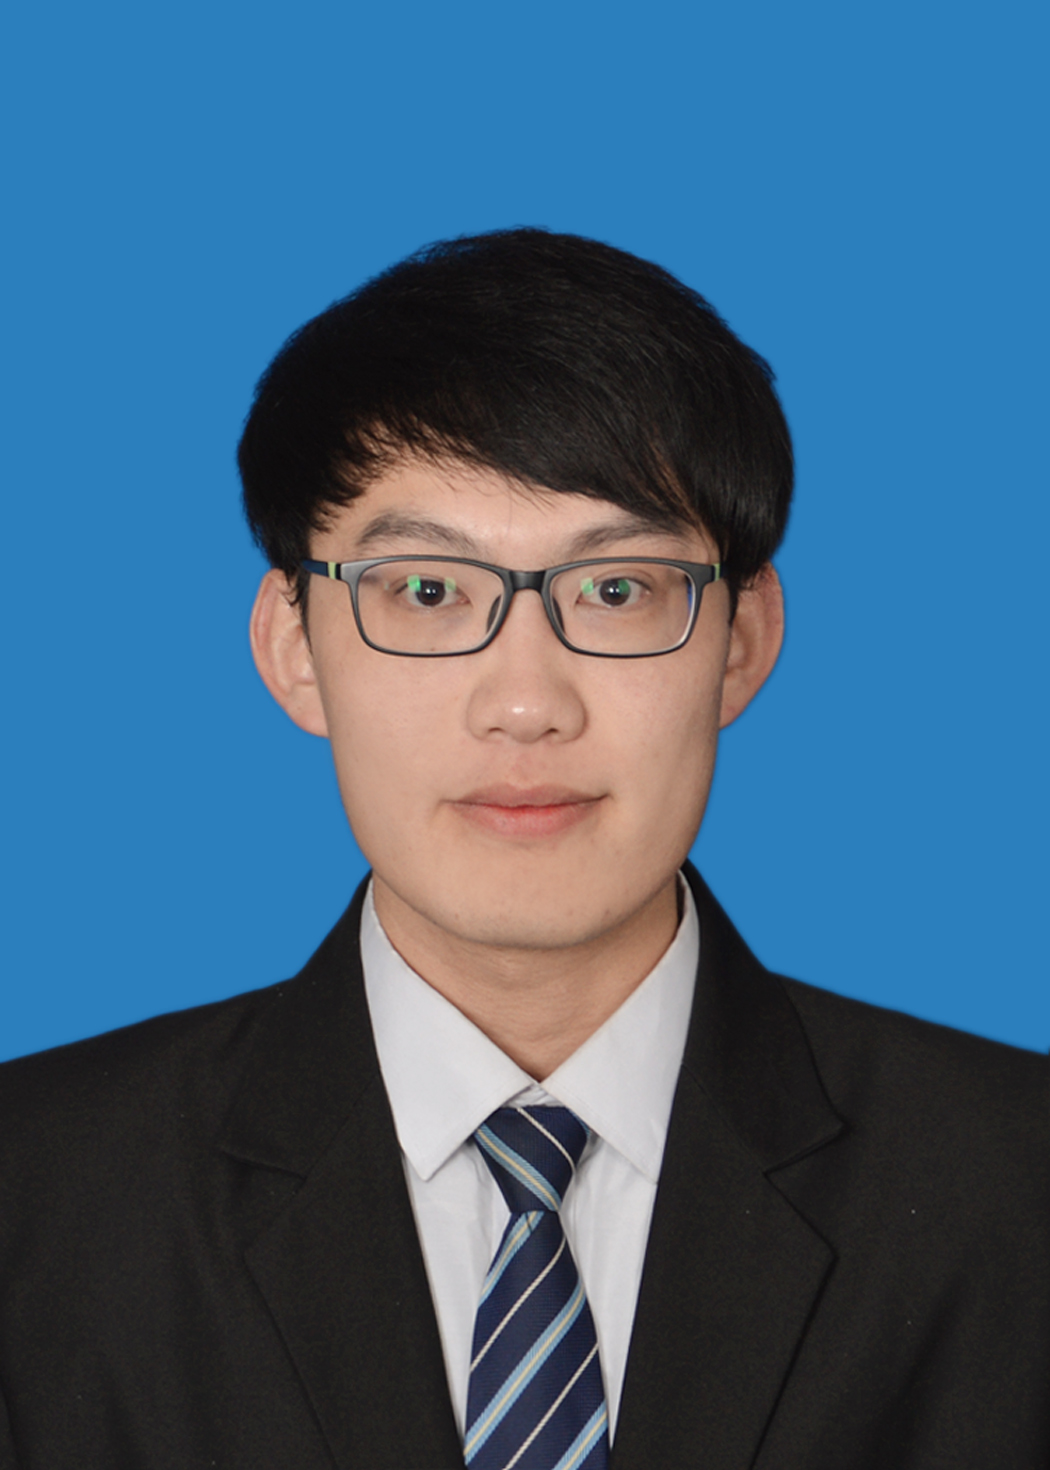
\includegraphics[width=1in,height=1.25in,clip,keepaspectratio]{photo/jiangdong.jpg}}]{Dong Jiang}
    received the B.S. degree from the Department of Electronic Information Science and Technology, Shandong University of Science and Technology, Qindao, Shandong Province, China, in 2017. He received the master degree from the Department of Computer Science and Technology, East China Normal University, Shanghai, China, in 2019. His current research interests are in computer networks.
\end{IEEEbiography}

\begin{IEEEbiography}[{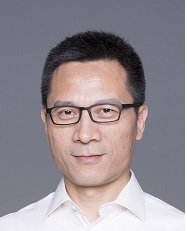
\includegraphics[width=1in,height=1.25in,clip,keepaspectratio]{photo/tongquanwei.jpg}}]{Tongquan Wei(M'11-SM'19)}
    received his Ph.D. degree in Electrical Engineering from Michigan Technological University in 2009. He is currently an Associate Professor in the Department of Computer Science and Technology at East China Normal University. His research interests are in the areas of internet of things (IoT), edge computing, cloud computing, and design automation of intelligent systems and cyber physical systems (CPS). He has published numerous papers in these areas, most of which are published in premium conferences and journals. He serves as a Regional Editor for Journal of Circuits, Systems, and Computers since 2012. He also served as the Guest Editor of the IEEE TII SS on Building Automation, Smart Homes, and Communities, the ACM TESC SS on Embedded Systems for Energy-Efficient, Reliable, and Secure Smart Homes, and the ACM TCPS SS on Human-Interaction-Aware Data Analytics for Cyber-Physical Systems. He is a senior member of the IEEE.
\end{IEEEbiography}

\begin{IEEEbiography}[{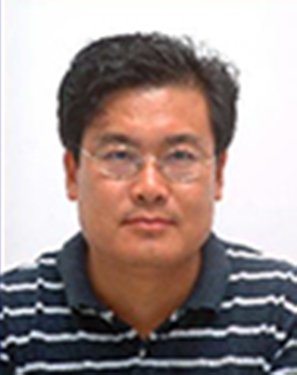
\includegraphics[width=1in,height=1.25in,clip,keepaspectratio]{photo/fukeshen.jpg}}]{Fuke Shen}
    received his Ph.D. degree in Department of Computer Science and Technology of East China Normal University in 2011. He is currently an Professor in the Department of Computer Science and Technology at East China Normal University, and director of Information Center at East China Normal University. His research interests are in the areas of computer networks communication, next generation network architecture, network protocols and their implementation, network traffic monitoring and management, and digital campus network.
\end{IEEEbiography}

\EOD

\end{document}
